This appendix details further geometric, magnetic, and finite-element data for most magnetic computations found in this thesis. The data is presented as an annotated diagram, showing the geometry of any magnets, along with a table (if relevant) stating magnetic properties, number of mesh elements, and finite-element computation time.

\newpage
\section{Chapter \ref{chap:paper1}}
\subsection{Chamfered cuboidal magnet}
\begin{figure}[h!]
    \centering
		\tdplotsetmaincoords{70}{110}
		\tdplotsetrotatedcoords{0}{0}{0}
		\begin{tikzpicture}[scale = 0.7,tdplot_rotated_coords]
		
		\coordinate (p1b) at (0,1,5);
		\coordinate (p2b) at (0,3,5);
		\coordinate (p3b) at (0,6,3);
		\coordinate (p4b) at (0,6,-2);
		\coordinate (p5b) at (0,1,-2);
		\coordinate (p1f) at (5,1,5);
		\coordinate (p2f) at (5,3,5);
		\coordinate (p3f) at (5,6,3);
		\coordinate (p4f) at (5,6,-2);
		\coordinate (p5f) at (5,1,-2);
		
		\draw (p1b) -- (p2b) -- (p3b) -- (p4b);% -- (p5b) -- cycle;
		\draw (p1f) -- (p2f) -- (p3f) -- (p4f) -- (p5f) -- cycle;
		\draw (p1f) -- (p1b);
		\draw (p2f) -- (p2b);
		\draw (p3f) -- (p3b);
		\draw (p4f) -- (p4b);
		
		% Draw a coordinate system
		\draw[->] (5,10,-2) -- (7,10,-2);
		\draw[->] (5,10,-2) -- (5,12,-2);
		\draw[->] (5,10,-2) -- (5,10,0);
		\node at (8,10,-2) {\(x\)};
		\node at (5,12.5,-2) {\(y\)};
		\node at (5,10,0.25) {\(z\)};
		
		\draw[->,thick] (5,3.5,0.5) -- (5,3.5,2.5);
		\node (M1) at (5,4,1.5) {\textbf{M}};
		
		% Draw dimensions
		\draw[<->] (5,0,-2) -- (5,0,5);
		\node at (5,-1.1,1.5) {7 units};
		\draw[<->] (5,0,5) -- (0,0,5);
		\node at (1.75,-1.1,5) {5 units};
		\draw[<->] (-1,1,5) -- (-1,3,5);
		\node at (-2.3,1.9,5) {2 units};
		\draw[<->] (0,7,-2) -- (0,7,3);
		\node at (0,8.1,0.5) {5 units};
		\draw[<->] (7,1.25,-2) -- (7,6.25,-2);
		\node at (8.5,4.25,-2) {5 units};
		\end{tikzpicture}
\end{figure}
\begin{table}[h!]
    \centering
    \begin{tabular}{c|c}
        \multicolumn{2}{c}{\textbf{Magnetic parameters}} \\ \hline
        Remanent magnetisation direction & \(\left(0,0,1\right)\) \\
        Remanent magnetisation strength & \SI{1}{\tesla} \\
        Relative permeability & 1 \\ \hline\hline
        \multicolumn{2}{c}{\textbf{Finite-element simulation}} \\ \hline
        Approx. number of mesh elements & N/A \\
        Approx. computation time & N/A \\ \hline\hline
    \end{tabular}
\end{table}

\newpage
\subsection{Two cuboidal magnets used by Akoun and Yonnet}
\begin{figure}[h!]
\centering
		\tdplotsetmaincoords{70}{130}
		\begin{tikzpicture}[scale=0.25,tdplot_main_coords]
		\coordinate(b1) at (10,-6,3);
		\coordinate(b2) at (10,6,3);
		\coordinate(b3) at (-10,6,3);
		\coordinate(b4) at (-10,-6,3);
		\coordinate(b5) at (10,-6,-3);
		\coordinate(b6) at (10,6,-3);
		\coordinate(b7) at (-10,6,-3);
		
		\draw (b1) -- (b2) -- (b3) -- (b4) -- cycle;
		\draw (b5) -- (b6) -- (b7);
		\draw (b1) -- (b5);
		\draw (b2) -- (b6);
		\draw (b3) -- (b7);
		
		\coordinate(t1) at (2,-14,11);
		\coordinate(t2) at (2,6,11);
		\coordinate(t3) at (-10,6,11);
		\coordinate(t4) at (-10,-14,11);
		\coordinate(t5) at (2,-14,5);
		\coordinate(t6) at (2,6,5);
		\coordinate(t7) at (-10,6,5);
		
		\draw[fill=white] (t1) -- (t2) -- (t6) -- (t5);
		\draw[fill=white] (t2) -- (t3) -- (t7) -- (t6);
		\draw (t5) -- (t1) -- (t4) -- (t3);
		
		\coordinate(midpt) at (2,-4,8);
		\coordinate(end) at (12,-4,8);
		
		\node(A) at (0,6,0) {\text{A}};
		\node(B) at (-4,6,8) {\text{B}};
		
		% Draw axes
		\draw[->] (-10,20,0) -- (-4,20,0);
		\node at (-2,20,0) {\(x\)};
		\draw[->] (-10,20,0) -- (-10,26,0);
		\node at (-10,28,0) {\(y\)};
		\draw[->] (-10,20,0) -- (-10,20,6);
		\node at (-10,20,8) {\(z\)};
		
		% Draw dimensions
		% Top magnet
		\draw[<->] (4,-14,5) -- (4,-14,11);
		\node at (8,-14,9.5) {6mm};
		\draw[<->] (-12,-17,11) -- (0,-17,11);
		\node at (-8,-21,11) {12mm};
		\draw[<->] (-13,-15,11) -- (-13,5,11);
		\node at (-17,-7,11) {20mm};
		% Bottom magnet
		\draw[<->] (12,-6,-3) -- (12,-6,3);
		\node at (16,-6,1.5) {6mm};
		\draw[<->] (14,-4,-3) -- (14,8,-3);
		\node at (18,4,-3) {12mm};
		\draw[<->] (12,9,-3) -- (-8,9,-3);
		\node at (3,13,-3) {20mm};
		\end{tikzpicture}
\end{figure}
\begin{table}[h!]
    \centering
    \begin{tabular}{c|c}
        \multicolumn{2}{c}{\textbf{Magnetic parameters for magnet A}} \\ \hline
        Remanent magnetisation direction & \(\left(0,0,1\right)\) \\
        Remanent magnetisation strength & \SI{0.38}{\tesla} \\
        Relative permeability & 1 \\ \hline\hline
        \multicolumn{2}{c}{\textbf{Magnetic parameters for magnet B}} \\ \hline
        Remanent magnetisation direction & \(\left(0,0,1\right)\) \\
        Remanent magnetisation strength & \SI{0.38}{\tesla} \\
        Relative permeability & 1 \\ \hline\hline
        \multicolumn{2}{c}{\textbf{Finite-element simulation}} \\ \hline
        Approx. number of mesh elements & 17,000 \\
        Approx. computation time & 30-40 seconds \\ \hline\hline
    \end{tabular}
\end{table}

\newpage
\subsection{Two identical regular dodecahedron magnets}
\begin{figure}[h!]
\centering
		\tdplotsetmaincoords{70}{110}
		\begin{tikzpicture}[scale=65,tdplot_main_coords]
		\coordinate(p1t) at (0.026180,0.008506,0.005258);
		\coordinate(p2t) at (0.016181,-0.005257,-0.022270);
		\coordinate(p3t) at (0.009999,-0.013765,0.022270);
		\coordinate(p4t) at (0.000000,-0.027527,-0.005258);
		\coordinate(p5t) at (-0.000000,0.027527,0.005258);
		\coordinate(p6t) at (-0.009999,0.013765,-0.022270);
		\coordinate(p7t) at (-0.016181,0.005257,0.022270);
		\coordinate(p8t) at (-0.026180,-0.008506,-0.005258);
		\coordinate(p9t) at (0.016180,0.022271,-0.005256);
		\coordinate(p10t) at (0.010001,0.013765,-0.022270);
		\coordinate(p11t) at (-0.010001,-0.013765,0.022270);
		\coordinate(p12t) at (-0.016180,-0.022271,0.005256);
		\coordinate(p13t) at (0.016180,0.005257,0.022271);
		\coordinate(p14t) at (0.000001,-0.017012,-0.022271);
		\coordinate(p15t) at (-0.000001,0.017012,0.022271);
		\coordinate(p16t) at (-0.016180,-0.005257,-0.022271);
		\coordinate(p17t) at (0.026180,-0.008506,-0.005257);
		\coordinate(p18t) at (0.016180,-0.022271,0.005257);
		\coordinate(p19t) at (-0.016180,0.022271,-0.005257);
		\coordinate(p20t) at (-0.026180,0.008506,0.005257);
		
		\coordinate(p1b) at (0.016180,0.022270,-0.049242);
		\coordinate(p2b) at (0.016180,0.005258,-0.076770);
		\coordinate(p3b) at (0.016180,-0.005258,-0.032230);
		\coordinate(p4b) at (0.016180,-0.022270,-0.059758);
		\coordinate(p5b) at (-0.016180,0.022270,-0.049242);
		\coordinate(p6b) at (-0.016180,0.005258,-0.076770);
		\coordinate(p7b) at (-0.016180,-0.005258,-0.032230);
		\coordinate(p8b) at (-0.016180,-0.022270,-0.059758);
		\coordinate(p9b) at (0.000000,0.027528,-0.059756);
		\coordinate(p10b) at (0.000000,0.017014,-0.076770);
		\coordinate(p11b) at (0.000000,-0.017014,-0.032230);
		\coordinate(p12b) at (0.000000,-0.027528,-0.049244);
		\coordinate(p13b) at (0.010000,0.013763,-0.032229);
		\coordinate(p14b) at (0.010000,-0.013763,-0.076771);
		\coordinate(p15b) at (-0.010000,0.013763,-0.032229);
		\coordinate(p16b) at (-0.010000,-0.013763,-0.076771);
		\coordinate(p17b) at (0.026180,0.008507,-0.059757);
		\coordinate(p18b) at (0.026180,-0.008507,-0.049243);
		\coordinate(p19b) at (-0.026180,0.008507,-0.059757);
		\coordinate(p20b) at (-0.026180,-0.008507,-0.049243);
		
		\draw[fill=white] (p3b) -- (p11b) -- (p7b) -- (p15b) -- (p13b) -- cycle;
		\draw[fill=white] (p11b) -- (p12b) -- (p4b) -- (p18b) -- (p3b) -- cycle;
		\draw[fill=white] (p3b) -- (p13b) -- (p1b) -- (p17b) -- (p18b) -- cycle;
		\draw[fill=white] (p13b) -- (p15b) -- (p5b) -- (p9b) -- (p1b) -- cycle;
		\draw[fill=white] (p18b) -- (p17b) -- (p2b) -- (p14b) -- (p4b) -- cycle;
		\draw[fill=white] (p1b) -- (p17b) -- (p2b) -- (p10b) -- (p9b) -- cycle;
		
		\draw[fill=white] (p11t) -- (p3t) -- (p13t) -- (p15t) -- (p7t) -- cycle;
		\draw[fill=white] (p3t) -- (p18t) -- (p17t) -- (p1t) -- (p13t) -- cycle;
		\draw[fill=white] (p1t) -- (p9t) -- (p5t) -- (p15t) -- (p13t) -- cycle;
		\draw[fill=white] (p1t) -- (p9t) -- (p10t) -- (p2t) -- (p17t) -- cycle;
		\draw[fill=white] (p18t) -- (p17t) -- (p2t) -- (p14t) -- (p4t) -- cycle;
		\draw[fill=white] (p9t) -- (p5t) -- (p19t) -- (p6t) -- (p10t) -- cycle;
		
		\node(A) at (0,0,-0.0525) {\text{A}};
		\node(B) at (0,0.012,0.005) {\text{B}};
		
		% Draw axes
		\draw[->] (0,0.07,-0.02) -- (0.025,0.07,-0.02);
		\node at (0.035,0.07,-0.02) {\(x\)};
		\draw[->] (0,0.07,-0.02) -- (0,0.095,-0.02);
		\node at (0,0.1,-0.02) {\(y\)};
		\draw[->] (0,0.07,-0.02) -- (0,0.07,0.005);
		\node at (0,0.07,0.01) {\(z\)};
		
		% Draw one dimension thingy
		\draw[<->] (-0.010001,-0.013765,0.027270) -- (-0.016181,0.005257,0.027270);
		\node at (-0.015,-0.005,0.032270) {20mm};
		\end{tikzpicture}
\end{figure}
\begin{table}[h!]
    \centering
    \begin{tabular}{c|c}
        \multicolumn{2}{c}{\textbf{Magnetic parameters for magnet A}} \\ \hline
        Remanent magnetisation direction & \(\left(0,0,1\right)\) \\
        Remanent magnetisation strength & \SI{1}{\tesla} \\
        Relative permeability & 1 \\ \hline\hline
        \multicolumn{2}{c}{\textbf{Magnetic parameters for magnet B}} \\ \hline
        Remanent magnetisation direction & \(\left(1,0,0\right)\) \\
        Remanent magnetisation strength & \SI{1}{\tesla} \\
        Relative permeability & 1 \\ \hline\hline
        \multicolumn{2}{c}{\textbf{Finite-element simulation}} \\ \hline
        Approx. number of mesh elements & 18,000 \\
        Approx. computation time & 40-50 seconds \\ \hline\hline
    \end{tabular}
\end{table}

\newpage
\section{Chapter \ref{chap:paper2}}
\subsection{Pyramid frustum magnet}
\begin{figure}[h!]
\centering
\def\lim{13}

\tdplotsetmaincoords{70}{45}
\begin{tikzpicture}[scale=0.13,tdplot_main_coords]

% Define coordinates:
\coordinate(ppb) at (15,15,-20);
\coordinate(pnb) at (15,-15,-20);
\coordinate(nnb) at (-15,-15,-20);
\coordinate(npb) at (-15,15,-20);
\coordinate(ppt) at (10,10,0);
\coordinate(pnt) at (10,-10,0);
\coordinate(nnt) at (-10,-10,0);
\coordinate(npt) at (-10,10,0);

% Fill in polygons:
\filldraw[fill=white] (ppt) -- (pnt) -- (nnt) -- (npt) -- cycle;
\filldraw[fill=white] (ppt) -- (ppb) -- (pnb) -- (pnt) -- cycle;
\filldraw[fill=white] (pnt) -- (nnt) -- (nnb) -- (pnb) -- cycle;

% Axes:
\draw[->] (0,0,0) -- (\lim,0,0);
\draw[->] (0,0,0) -- (0,\lim,0);
\draw[->] (0,0,0) -- (0,0,\lim);
\node(xaxis) at (\lim+2,0,0) {\(x\)};
\node(yaxis) at (0,\lim+2,0) {\(y\)};
\node(zaxis) at (0,0,\lim+2) {\(z\)};

% Dimensions:
\draw[<->] (20,-18,-20) -- (20,12,-20);
\node(botdim) at (26,-5,-20) {30mm};
\draw[<->] (-12,-20,-20) -- (18,-20,-20);
\node(botdim2) at (5,-26,-20) {30mm};
\draw[<->] (-15,-7,0) -- (-15,13,0);
\node(topdim) at (-21,6,0) {20mm};
\draw[<->] (-6,-15,0) -- (14,-15,0);
\node(topdim2) at (6,-21,0) {20mm};
\draw[<->] (17,17,-20) -- (17,17,0);
\node(height) at (21,21,-10) {20mm};

\end{tikzpicture}
\end{figure}
\begin{table}[h!]
    \centering
    \begin{tabular}{c|c}
        \multicolumn{2}{c}{\textbf{Magnetic parameters}} \\ \hline
        Remanent magnetisation direction & \(\left(0,0,1\right)\) \\
        Remanent magnetisation strength & \SI{1.3}{\tesla} \\
        Relative permeability & 1 \\ \hline\hline
        \multicolumn{2}{c}{\textbf{Finite-element simulation}} \\ \hline
        Approx. number of mesh elements & 1,200,000 \\
        Approx. computation time & 41 minutes \\ \hline\hline
    \end{tabular}
\end{table}

\newpage
\subsection{Cylindrical magnet}
\begin{figure}[h!]
\centering
\def\lim{13}

\tdplotsetmaincoords{70}{0}
\begin{tikzpicture}[scale=0.14,tdplot_main_coords]

% Draw cylinder
\draw (-10,0,-20) arc[radius = 10, start angle = -180, end angle = 0];
\draw (0,0,0) circle [radius = 10];
\draw (-10,0,0) -- (-10,0,-20);
\draw (10,0,0) -- (10,0,-20);

% Axes:
\draw[->] (0,0,0) -- (\lim,0,0);
\draw[->] (0,0,0) -- (0,0,\lim);
\node(xaxis) at (\lim+2,0,0) {\(x\)};
\node(zaxis) at (0,0,\lim+2) {\(z\)};

% Dimensions:
\draw[<->] (0,0,-27) -- (10,0,-27);
\node(radius) at (5,0,-30) {10mm};
\draw[<->] (-15,0,-20) -- (-15,0,0);
\node(height) at (-20,0,-10) {20mm};

\end{tikzpicture}
\end{figure}
\begin{table}[h!]
    \centering
    \begin{tabular}{c|c}
        \multicolumn{2}{c}{\textbf{Magnetic parameters}} \\ \hline
        Remanent magnetisation direction & \(\left(0,0,1\right)\) \\
        Remanent magnetisation strength & \SI{1.3}{\tesla} \\
        Relative permeability & 1 \\ \hline\hline
        \multicolumn{2}{c}{\textbf{Finite-element simulation}} \\ \hline
        Approx. number of mesh elements & 960,000 \\
        Approx. computation time & 38 minutes \\ \hline\hline
    \end{tabular}
\end{table}

\newpage
\section{Chapter \ref{chap:paper3}}
\subsection{Cube magnet}
\begin{figure}[h!]
\centering
\def\lim{13}

\tdplotsetmaincoords{70}{45}
\begin{tikzpicture}[scale=0.13,tdplot_main_coords]

% Define coordinates:
\coordinate(ppb) at (10,10,-20);
\coordinate(pnb) at (10,-10,-20);
\coordinate(nnb) at (-10,-10,-20);
\coordinate(npb) at (-10,10,-20);
\coordinate(ppt) at (10,10,0);
\coordinate(pnt) at (10,-10,0);
\coordinate(nnt) at (-10,-10,0);
\coordinate(npt) at (-10,10,0);

% Fill in polygons:
\filldraw[fill=white] (ppt) -- (pnt) -- (nnt) -- (npt) -- cycle;
\filldraw[fill=white] (ppt) -- (ppb) -- (pnb) -- (pnt) -- cycle;
\filldraw[fill=white] (pnt) -- (nnt) -- (nnb) -- (pnb) -- cycle;

% Axes:
\draw[->] (0,0,0) -- (\lim,0,0);
\draw[->] (0,0,0) -- (0,\lim,0);
\draw[->] (0,0,0) -- (0,0,\lim);
\node(xaxis) at (\lim+2,0,0) {\(x\)};
\node(yaxis) at (0,\lim+2,0) {\(y\)};
\node(zaxis) at (0,0,\lim+2) {\(z\)};

% Dimensions:
\draw[<->] (20,-13,-20) -- (20,7,-20);
\node(botdim) at (26,-5,-20) {\(l\)};
\draw[<->] (-7,-20,-20) -- (13,-20,-20);
\node(botdim2) at (5,-26,-20) {\(l\)};
\draw[<->] (14,14,-20) -- (14,14,0);
\node(height) at (16,16,-10) {\(l\)};

\end{tikzpicture}
\end{figure}
\begin{table}[h!]
    \centering
    \begin{tabular}{c|c}
        \multicolumn{2}{c}{\textbf{Magnetic parameters}} \\ \hline
        Remanent magnetisation direction & \(\left(0,0,1\right)\) \\
        Remanent magnetisation strength & N/A \\
        Relative permeability & 1 \\ \hline\hline
        \multicolumn{2}{c}{\textbf{Finite-element simulation}} \\ \hline
        Approx. number of mesh elements & N/A \\
        Approx. computation time & N/A \\ \hline\hline
    \end{tabular}
\end{table}

\newpage
\subsection{Optimal cuboid}
\begin{figure}[h!]
\centering
\def\lim{13}

\tdplotsetmaincoords{70}{45}
\begin{tikzpicture}[scale=0.13,tdplot_main_coords]

% Define coordinates:
\coordinate(ppb) at (8.13,8.13,-30.28);
\coordinate(pnb) at (8.13,-8.13,-30.28);
\coordinate(nnb) at (-8.13,-8.13,-30.28);
\coordinate(npb) at (-8.13,8.13,-30.28);
\coordinate(ppt) at (8.13,8.13,0);
\coordinate(pnt) at (8.13,-8.13,0);
\coordinate(nnt) at (-8.13,-8.13,0);
\coordinate(npt) at (-8.13,8.13,0);

% Fill in polygons:
\filldraw[fill=white] (ppt) -- (pnt) -- (nnt) -- (npt) -- cycle;
\filldraw[fill=white] (ppt) -- (ppb) -- (pnb) -- (pnt) -- cycle;
\filldraw[fill=white] (pnt) -- (nnt) -- (nnb) -- (pnb) -- cycle;

% Axes:
\draw[->] (0,0,0) -- (\lim,0,0);
\draw[->] (0,0,0) -- (0,\lim,0);
\draw[->] (0,0,0) -- (0,0,\lim);
\node(xaxis) at (\lim+2,0,0) {\(x\)};
\node(yaxis) at (0,\lim+2,0) {\(y\)};
\node(zaxis) at (0,0,\lim+2) {\(z\)};

% Dimensions:
\draw[<->] (18,-11.13,-30.28) -- (18,5.13,-30.28);
\node(botdim) at (25,-7,-30.28) {\(0.813l\)};
\draw[<->] (-5.13,-18,-30.28) -- (11.13,-18,-30.28);
\node(botdim2) at (7,-25,-30.28) {\(0.813l\)};
\draw[<->] (13,13,-30.28) -- (13,13,0);
\node(height) at (16,16,-15) {\(1.514l\)};

\end{tikzpicture}
\end{figure}
\begin{table}[h!]
    \centering
    \begin{tabular}{c|c}
        \multicolumn{2}{c}{\textbf{Magnetic parameters}} \\ \hline
        Remanent magnetisation direction & \(\left(0,0,1\right)\) \\
        Remanent magnetisation strength & N/A \\
        Relative permeability & 1 \\ \hline\hline
        \multicolumn{2}{c}{\textbf{Finite-element simulation}} \\ \hline
        Approx. number of mesh elements & N/A \\
        Approx. computation time & N/A \\ \hline\hline
    \end{tabular}
\end{table}

\newpage
\subsection{Optimal frustum}
\begin{figure}[h!]
\centering
\def\lim{13}

\tdplotsetmaincoords{70}{45}
\begin{tikzpicture}[scale=0.13,tdplot_main_coords]

% Define coordinates:
\coordinate(ppb) at (15.8,15.8,-19.02);
\coordinate(pnb) at (15.8,-15.8,-19.02);
\coordinate(nnb) at (-15.8,-15.8,-19.02);
\coordinate(npb) at (-15.8,15.8,-19.02);
\coordinate(ppt) at (3.44,3.44,0);
\coordinate(pnt) at (3.44,-3.44,0);
\coordinate(nnt) at (-3.44,-3.44,0);
\coordinate(npt) at (-3.44,3.44,0);

% Fill in polygons:
\filldraw[fill=white] (ppt) -- (pnt) -- (nnt) -- (npt) -- cycle;
\filldraw[fill=white] (ppt) -- (ppb) -- (pnb) -- (pnt) -- cycle;
\filldraw[fill=white] (pnt) -- (nnt) -- (nnb) -- (pnb) -- cycle;

% Axes:
\draw[->] (0,0,0) -- (\lim,0,0);
\draw[->] (0,0,0) -- (0,\lim,0);
\draw[->] (0,0,0) -- (0,0,\lim);
\node(xaxis) at (\lim+2,0,0) {\(x\)};
\node(yaxis) at (0,\lim+2,0) {\(y\)};
\node(zaxis) at (0,0,\lim+2) {\(z\)};

% Dimensions:
\draw[<->] (20,-18.8,-20) -- (20,12.8,-20);
\node(botdim) at (26,-5,-20) {\(1.580l\)};
\draw[<->] (-12.8,-20,-20) -- (18.8,-20,-20);
\node(botdim2) at (5,-26,-20) {\(1.580l\)};
\draw[<->] (-10,-0.44,0) -- (-10,6.44,0);
\node(topdim) at (-18,6,0) {\(0.344l\)};
\draw[<->] (-0.44,-10,0) -- (6.44,-10,0);
\node(topdim2) at (9,-17,0) {\(0.344l\)};
\draw[<->] (18,18,-19.02) -- (18,18,0);
\node(height) at (21,21,-10) {\(0.951l\)};

\end{tikzpicture}
\end{figure}
\begin{table}[h!]
    \centering
    \begin{tabular}{c|c}
        \multicolumn{2}{c}{\textbf{Magnetic parameters}} \\ \hline
        Remanent magnetisation direction & \(\left(0,0,1\right)\) \\
        Remanent magnetisation strength & N/A \\
        Relative permeability & 1 \\ \hline\hline
        \multicolumn{2}{c}{\textbf{Finite-element simulation}} \\ \hline
        Approx. number of mesh elements & N/A \\
        Approx. computation time & N/A \\ \hline\hline
    \end{tabular}
\end{table}

\newpage
\section{Chapter \ref{chap:paper4}}
\subsection{Cube magnets in repulsion}
\begin{figure}[h!]
\centering
\begin{tikzpicture}

% Set up coordinates of vertices
\coordinate(toptl) at (-1,3);
\coordinate(toptr) at (1,3);
\coordinate(topbl) at (-1,1);
\coordinate(topbr) at (1,1);
\coordinate(bottl) at (-1,0);
\coordinate(bottr) at (1,0);
\coordinate(botbl) at (-1,-2);
\coordinate(botbr) at (1,-2);

% Draw magnets
\draw (toptl) -- (toptr) -- (topbr) -- (topbl) -- cycle;
\draw (bottl) -- (bottr) -- (botbr) -- (botbl) -- cycle;

% Draw magnetisation vectors
\draw[->,thick] (0,2.5) -- (0,1.5);
\draw[->,thick] (0,-1.5) -- (0,-0.5);
\node(Mtop) at (0.5,2) {\(\mathbf{B}_{r\text{,top}}\)};
\node(Mbot) at (0.5,-1) {\(\mathbf{B}_{r\text{,bot}}\)};

% Draw dimensions
\draw[<->] (2,3) -- (2,1);
\node(lsidetop) at (2.7,2) {10mm};
\draw[<->] (-2,1) -- (-2,0);
\node(d) at (-1.7,0.5) {\(d\)};
\draw[<->] (2,0) -- (2,-2);
\node(lsidebot) at (2.7,-1) {10mm};
\draw[<->] (-1,-3) -- (1,-3);
\node(lunder) at (0,-2.7) {10mm};

% Draw a coordinate system
\draw[->] (-4,-1) -- (-3,-1);
\node at (-2.75,-1) {\(x\)};
\draw[->] (-4,-1) -- (-4,0);
\node at (-4,0.25) {\(z\)};

\end{tikzpicture}
\end{figure}
\begin{table}[h!]
    \centering
    \begin{tabular}{c|c}
        \multicolumn{2}{c}{\textbf{Magnetic parameters for top magnet}} \\ \hline
        Remanent magnetisation direction & \(\left(0,0,-1\right)\) \\
        Remanent magnetisation strength & \SI{1}{\tesla} \\
        Relative permeability & 1, 1.05, 1.2, or 3 \\ \hline\hline
        \multicolumn{2}{c}{\textbf{Magnetic parameters for bottom magnet}} \\ \hline
        Remanent magnetisation direction & \(\left(0,0,1\right)\) \\
        Remanent magnetisation strength & \SI{1}{\tesla} \\
        Relative permeability & 1, 1.05, 1.2, or 3 \\ \hline\hline
        \multicolumn{2}{c}{\textbf{Finite-element simulation}} \\ \hline
        Approx. number of mesh elements & 58,000 \\
        Approx. computation time & 60-70 seconds \\ \hline\hline
    \end{tabular}
\end{table}

\newpage
\subsection{Cube magnets with one rotating}
\begin{figure}[h!]
\centering
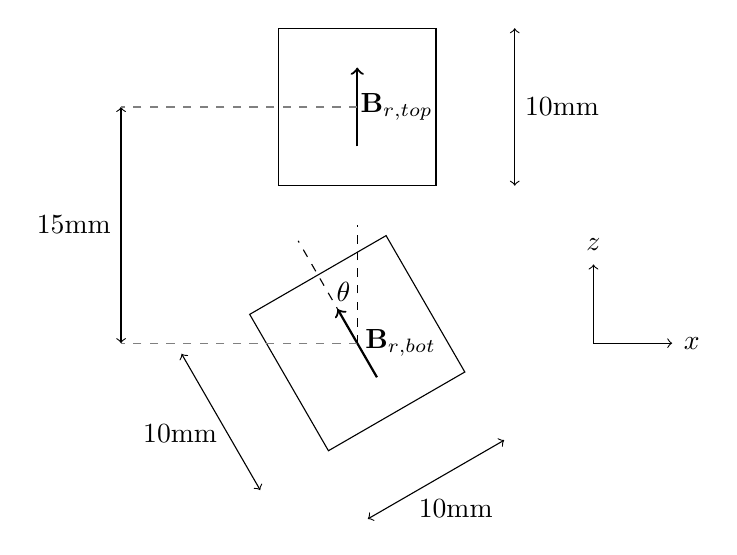
\begin{tikzpicture}
% Set up coordinates of vertices
\coordinate(toptl) at (-1,4);
\coordinate(toptr) at (1,4);
\coordinate(topbl) at (-1,2);
\coordinate(topbr) at (1,2);
\coordinate(bottl) at (0.366,1.366);
\coordinate(bottr) at (-1.366,0.366);
\coordinate(botbl) at (1.366,-0.366);
\coordinate(botbr) at (-0.366,-1.366);

% Draw magnets
\draw (toptl) -- (toptr) -- (topbr) -- (topbl) -- cycle;
\draw (bottl) -- (bottr) -- (botbr) -- (botbl) -- cycle;

% Draw magnetisation vectors
\draw[->,thick] (0,2.5) -- (0,3.5);
\draw[->,thick] (0.25,-0.433) -- (-0.25,0.433);
\node(Mtop) at (0.5,3) {\(\mathbf{B}_{r\text{,top}}\)};
\node(Mbot) at (0.55,-0) {\(\mathbf{B}_{r\text{,bot}}\)};

% Draw dimensions
\draw[<->] (2,2) -- (2,4);
\node(lsidetop) at (2.6,3) {10mm};
\draw[<->] (-2.232,-0.134) -- (-1.232,-1.866);
\node(lsidebot) at (-2.25,-1.15) {10mm};
\draw[<->] (1.866,-1.232) -- (0.134,-2.232);
\node(lunder) at (1.25,-2.1) {10mm};
\draw[<->] (-3,0) -- (-3,3);
\node(d) at (-3.6,1.5) {15mm};

% Draw horizontal centrelines
\draw[dashed,gray] (0,3) -- (-3,3);
\draw[dashed,gray] (0,0) -- (-3,0);

% Draw a coordinate system
\draw[->] (3,0) -- (4,0);
\node at (4.25,0) {\(x\)};
\draw[->] (3,0) -- (3,1);
\node at (3,1.25) {\(z\)};

% Draw angle
\draw[dashed] (0,0) -- (0,1.5);
\draw[dashed] (0,0) -- (-0.75,1.3);
\node(theta) at (-0.175,0.65) {\(\theta\)};
\end{tikzpicture}
\end{figure}
\begin{table}[h!]
    \centering
    \begin{tabular}{c|c}
        \multicolumn{2}{c}{\textbf{Magnetic parameters for top magnet}} \\ \hline
        Remanent magnetisation direction & \(\left(0,0,1\right)\) \\
        Remanent magnetisation strength & \SI{1}{\tesla} \\
        Relative permeability & 1, 1.05, 1.2, or 3 \\ \hline\hline
        \multicolumn{2}{c}{\textbf{Magnetic parameters for bottom magnet}} \\ \hline
        Remanent magnetisation direction & \(\left(-\sin\theta, 0, \cos\theta\right)\) \\
        Remanent magnetisation strength & \SI{1}{\tesla} \\
        Relative permeability & 1, 1.05, 1.2, or 3 \\ \hline\hline
        \multicolumn{2}{c}{\textbf{Finite-element simulation}} \\ \hline
        Approx. number of mesh elements & 58,000 \\
        Approx. computation time & 60-70 seconds \\ \hline\hline
    \end{tabular}
\end{table}